\section{Component Interfaces}

As shown in \textit{Section 2.4}, many method are invoked on the interfaces. Their interactions guarantee the execution of the most important processes required to fulfill DREAM's goals.\\
The following diagram is presented to better understand how interfaces interact with each other. \\
The methods listed in the  diagram are a logical representation of what component interfaces have to guarantee the users. \\
Certainly, considering a future implementation, they will be subjected to many modifications, according to choices and needs of developers. 

\def\fillandplacepagenumber{%
 \par\pagestyle{empty}%
\vbox to 0pt{\vss}\vfill
\vbox to 0pt{\baselineskip0pt
   \hbox to\linewidth{\hss}%
   \setlength{\footskip}{70pt}
   \baselineskip\footskip
   \hbox to\linewidth{%
     \hfil\thepage\hfil}\vss}}

\begin{landscape}
\begin{figure}[h]
\vspace*{-2cm}
\noindent
\centering
\centerline{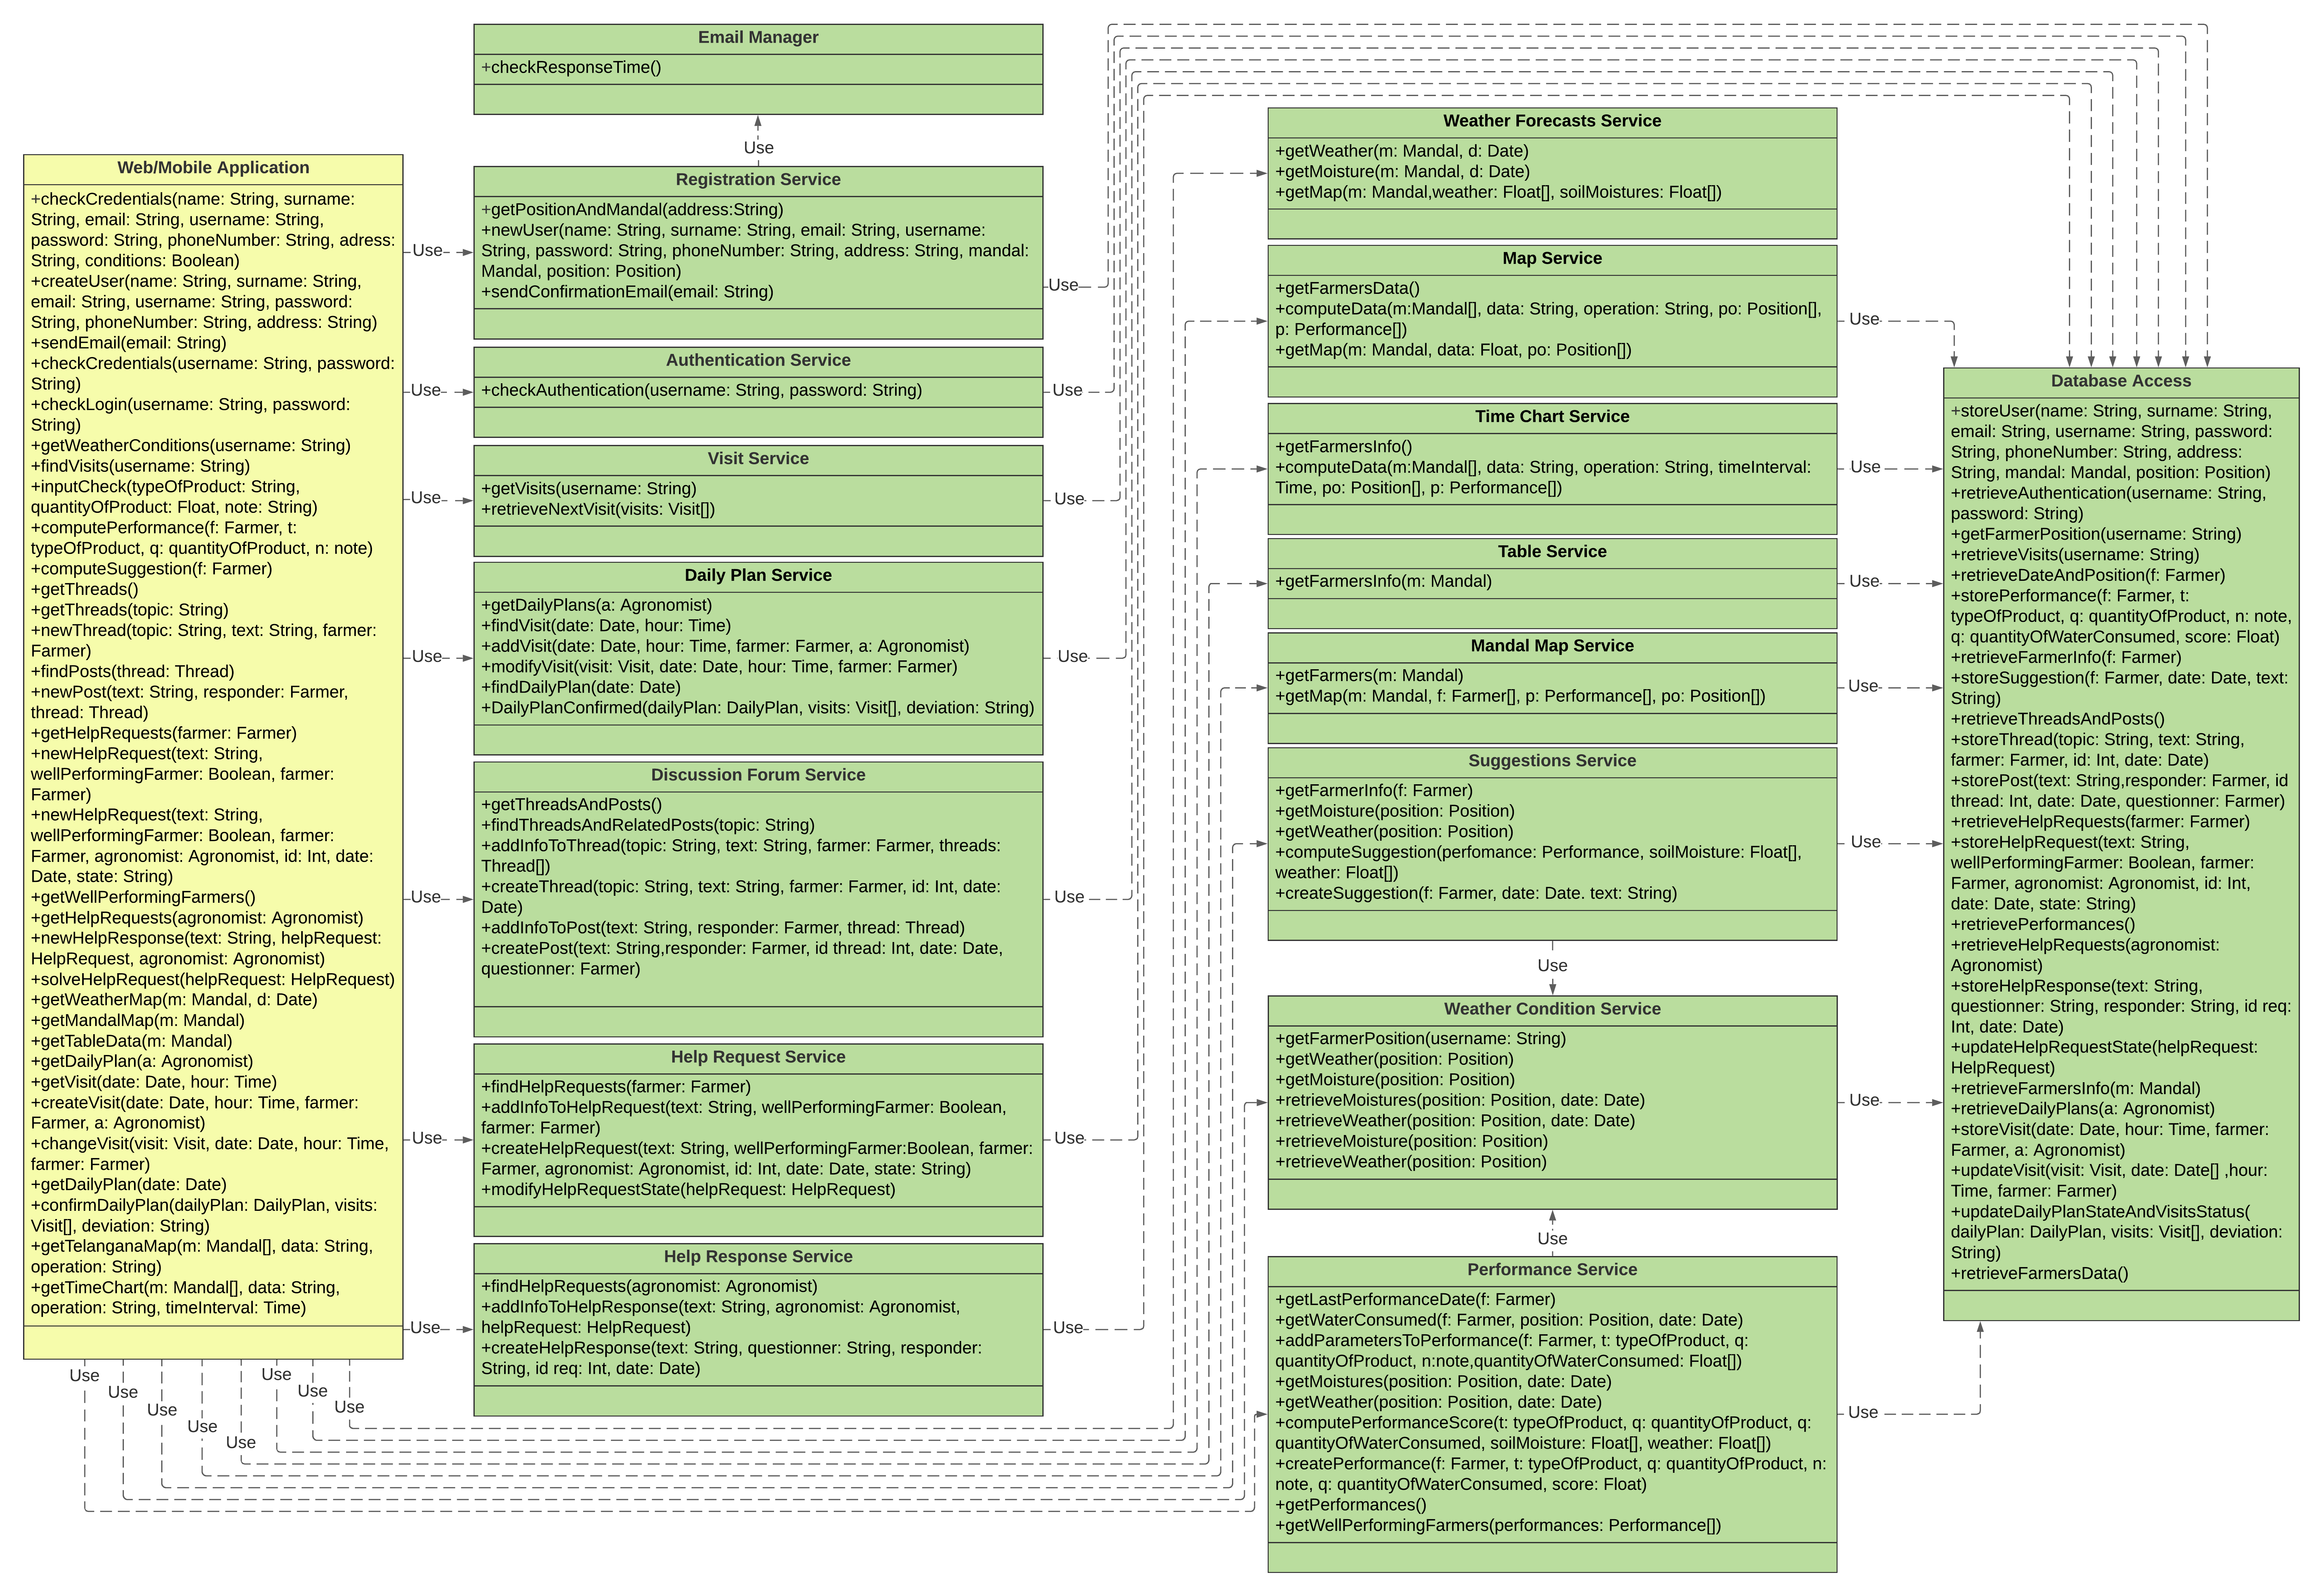
\includegraphics[scale = 0.09]{./Images/Component Interfaces.png}}
\vspace*{-1cm}
    \caption{Component Interfaces diagram}
    \vspace*{-12cm}
\end{figure}
\fillandplacepagenumber
\end{landscape}